% begin module sequence-limit-def
\begin{frame}
\begin{definition}[Limit of a Sequence]
A sequence $\{ a_n\}$ has the limit $L$, and we write
\[
\lim_{n\to\infty}a_n = L \qquad \textrm{or}\qquad a_n\to L \ \textrm{as} \ n\to \infty
\]
if we can make $a_n$ as close to $L$ as we like by taking $n$ large enough.
\end{definition}
\begin{definition}[Convergent]
A sequence that has a limit is called convergent.  A sequence that has no limit is called divergent.
\end{definition}
\begin{columns}[c]
\column{.5\textwidth}
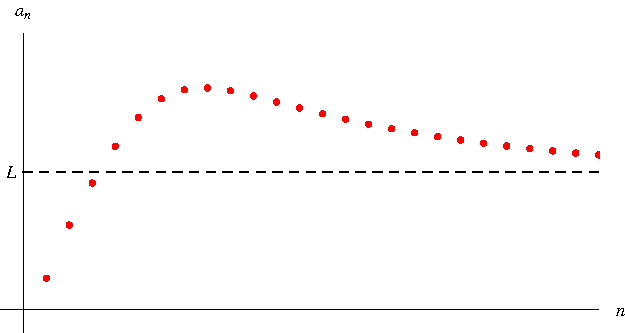
\includegraphics[width=6cm]{sequences/pictures/12-01-limita.pdf}%
\column{.5\textwidth}
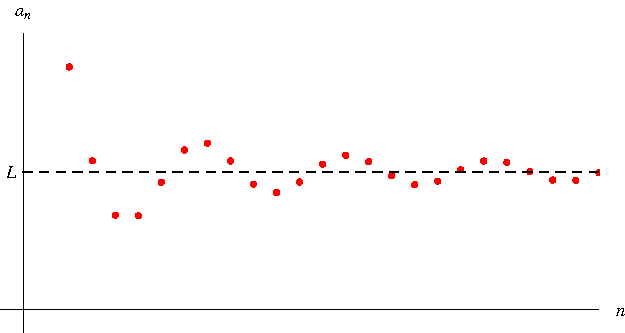
\includegraphics[width=6cm]{sequences/pictures/12-01-limitb.pdf}%
\end{columns}
\end{frame}
% end module sequence-limit-def
